\documentclass[runningheads]{llncs}

\usepackage{graphicx}
\usepackage{booktabs}
\usepackage{url}

\begin{document}

\title{Deterministic Parallel Transaction Execution for Logos Execution Zone: A Comparative and Experimental Study}
\titlerunning{Deterministic Parallel Transaction Execution for LEZ}

\author{Daniel Garbanzo}
\authorrunning{D. Garbanzo}
\institute{Instituto Tecnologico de Costa Rica\\
Master's Program in Computer Science -- Parallel Computing (MC-8836)}

\maketitle

\begin{abstract}
Modern blockchain execution layers must increase transaction throughput without changing deterministic state-machine semantics. A central challenge is that transactions in an ordered block may access shared state such as accounts, nonces, storage keys, nullifiers, commitments, and program metadata. This paper presents CAPE, a Conflict-Aware Parallel Executor model for studying deterministic parallel transaction execution using Logos Execution Zone as the main architectural case study. CAPE defines a common transaction and conflict model and compares three strategies: sequential execution, static conflict-aware batching, and optimistic execution with ordered commit and re-execution. The Rust prototype generates controlled workloads with disjoint access, hotspot contention, Zipfian popularity, token transfers, and simplified private-state operations. Across 990 benchmark rows, including 360 local rows on an Apple M2 Pro and 630 Kabré rows on a Dribe Xeon node with 36 allocated CPUs, all parallel executions matched the sequential final state hash and per-transaction outcomes. The optimistic executor achieved the best measured local throughput, 731,729.63 transactions per second, on a no-conflict workload with 8 threads and 5,000 transactions per block. The Kabré run reached 583,276.55 transactions per second on the same workload family with 16 threads, validating correctness and high-thread stress behavior but not exceeding the local peak. Static scheduling was useful only when batches remained large, but barrier-like workloads collapsed into small batches. The main contributions are a comparative taxonomy of blockchain parallel execution techniques, a Logos-oriented conflict model, a reproducible Rust benchmark, and a practical adaptation path for LEZ that starts from safe parallel validation and ordered state-diff commit.
\keywords{Parallel computing \and Blockchain execution \and Determinism \and Scheduling \and Optimistic concurrency control \and Logos Execution Zone}
\end{abstract}

\section{Introduction}

Blockchain nodes implement replicated state machines. Given the same initial state and the same ordered block, honest nodes must compute the same final state. The simplest execution policy is sequential: validate and apply each transaction in canonical block order. This policy is easy to reason about and deterministic by construction, but it underuses multicore hardware and can limit throughput.

Modern blockchain systems expose several approaches to this problem. Solana Sealevel schedules transactions using declared account access metadata \cite{solana_sealevel_2019}. Aptos Block-STM adapts software transactional memory to ordered blockchain blocks \cite{gelashvili2022blockstm}. Cosmos SDK documents similar Block-STM integration concerns around serial equivalence and application-specific validation \cite{cosmos_blockstm_docs}. Monad preserves Ethereum-style ordered semantics while using optimistic execution and asynchronous execution \cite{monad_parallel_execution_docs,monad_async_execution_docs}. Sei describes an optimistic concurrency engine with dependency estimation and conflict resolution \cite{sei_parallelization_engine_docs}. Sui exposes independence through an object ownership model \cite{sui_object_ownership_docs}.

This paper studies these ideas from a parallel computing perspective and applies them to Logos Execution Zone (LEZ), a Rust-based programmable execution environment with public and private state \cite{logos_execution_zone_github}. LEZ is an appropriate case study because its execution model separates validation from state mutation: validation can produce state diffs that are later committed to public accounts, nonces, commitments, nullifiers, and program state. This structure suggests a two-phase design: perform safe validation or computation in parallel, then commit deterministic diffs in canonical order.

The project does not attempt to implement a production Logos node or compare directly against production systems whose internals are unavailable. Instead, it contributes a controlled prototype and evaluation. The contributions are:

\begin{enumerate}
\item a taxonomy of deterministic parallel blockchain execution strategies;
\item a common conflict model covering public accounts, nonces, read/write sets, nullifiers, commitments, program deployments, and system barriers;
\item a Logos-oriented case study identifying parallelizable validation and ordered-commit constraints;
\item CAPE, a reproducible Rust prototype comparing sequential, static conflict-aware, and optimistic ordered-commit execution;
\item an experimental evaluation under controlled workloads showing where parallel execution helps and where contention dominates.
\end{enumerate}

\section{Background and Related Work}

Parallel computing studies how work can be decomposed while managing synchronization, communication, load balance, and memory contention \cite{pacheco2011parallel}. Speedup is measured as $T_1/T_p$, and parallel efficiency is speedup divided by the number of workers. Amdahl-style limits appear when some fraction of work must remain serial. In CAPE, serial work includes ordered commit, validation of read versions, and unavoidable conflicts.

Bulk Synchronous Parallel (BSP) provides useful vocabulary for static batching: independent work is executed in a superstep, followed by synchronization and ordered commit \cite{valiant1990bsp}. LogP emphasizes that communication and synchronization overhead are not free \cite{culler1993logp}. Roofline modeling is not the evaluation method here, but it motivates distinguishing compute-heavy transactions from metadata-bound schedulers \cite{williams2009roofline}. To avoid measuring only framework overhead, the prototype supports configurable artificial compute cost.

Optimistic concurrency control (OCC) assumes conflicts are uncommon: transactions execute speculatively and validate before commit \cite{kung1981optimistic}. Software transactional memory applies related ideas to shared-memory programs by tracking read and write sets \cite{shavit1997stm}. Block-STM applies this approach to blockchain blocks with predetermined order, validating speculative reads and re-executing invalidated transactions \cite{gelashvili2022blockstm}. Earlier smart-contract concurrency work also explored optimistic and object-based transactional execution \cite{anjana2018optimistic_smart_contracts,anjana2019object_tm_smart_contracts,reijsbergen2020transaction_concurrency}.

Table~\ref{tab:taxonomy} summarizes the design points relevant to CAPE.

\begin{table}
\centering
\caption{Taxonomy of deterministic parallel blockchain execution strategies.}
\label{tab:taxonomy}
\resizebox{\textwidth}{!}{%
\begin{tabular}{llll}
\toprule
System & Dependency information & Strategy & Determinism policy\\
\midrule
Sequential & none & ordered execution & canonical by construction\\
Solana & declared accounts & static scheduling & account access metadata\\
Aptos & dynamic read/write sets & Block-STM & preset block order\\
Cosmos SDK & store tracking & Block-STM option & AppHash equivalence\\
Monad & tracked inputs & optimistic execution & Ethereum-equivalent order\\
Sei & estimated/runtime sets & OCC hybrid & deterministic resolution\\
Sui & object ownership & object-level independence & ownership constraints\\
Logos LEZ & accounts, diffs, nullifiers & case-study target & ordered state transition\\
\bottomrule
\end{tabular}
}
\end{table}

\section{Problem Description}

Let a block be
\[
B = [tx_1, tx_2, \ldots, tx_n]
\]
and let $S_0$ be the initial state. Canonical sequential execution defines
\[
S_i = apply(validate(tx_i, S_{i-1}))
\]
for each transaction $tx_i$. A parallel executor is correct only if
\[
parallel(B,S_0).state = sequential(B,S_0).state
\]
and
\[
parallel(B,S_0).outcomes = sequential(B,S_0).outcomes.
\]

The difficulty is that blockchain transactions access shared state. In a Logos-inspired model, conflicts may involve public account balances, signer nonces, storage keys, deployed program code, private nullifiers, commitment roots, commitment slots, system clocks, and global configuration. Some work is naturally parallel, such as stateless checks, signature verification, proof verification, and computation over snapshots. Other work must respect canonical order because it changes the replicated state.

This leads to four research questions:

\begin{enumerate}
\item How much speedup can static conflict-aware scheduling obtain under different contention patterns?
\item How does optimistic execution behave as conflict rate increases?
\item Which LEZ-inspired state components can be parallelized safely and which require ordered commit?
\item What overheads dominate when available parallelism is low?
\end{enumerate}

\section{CAPE: Conflict-Aware Parallel Executor}

CAPE is a controlled experimental model, not a production blockchain runtime. Its state model includes accounts, nonces, nullifiers, commitments, program code, program storage, a system clock, global configuration, and a per-key version map. Each conflict-relevant item is represented as a \texttt{StateKey}. Every write increments the version of the written key. A canonical state hash is computed over sorted state components, avoiding dependence on hash-map iteration order.

Transactions carry a kind, signer, optional receiver, declared reads, declared writes, consumed nullifiers, produced commitments, optional program identifiers, amount, and compute cost. The prototype implements five transaction families: public transfers, private transfers, program calls, program deployments, and system transactions. Rejected transactions produce no state diff but still produce deterministic outcomes.

\subsection{Conflict Relation}

Two transactions conflict when their effects cannot be reordered without potentially changing sequential semantics. CAPE uses the following rule:
\[
conflict(tx_i, tx_j) \Leftrightarrow
(W_i \cap W_j \neq \emptyset) \lor
(W_i \cap R_j \neq \emptyset) \lor
(R_i \cap W_j \neq \emptyset)
\]
with additional treatment for duplicate nullifiers, program deployment, system clock, and global configuration. System and deployment transactions are barriers.

\subsection{Execution Strategies}

\paragraph{Sequential baseline.}
The sequential executor clones the initial state, executes each transaction in block order, applies its diff, records the outcome, and computes the final hash. It is the correctness oracle.

\paragraph{Static conflict-aware scheduling.}
The static executor greedily builds batches from declared read/write sets. A transaction is added to the current batch only if it has no read/write or write/write overlap with the accumulated batch sets. Barrier transactions form single-transaction batches. Each batch executes in parallel over a snapshot and commits diffs in canonical order.

\paragraph{Optimistic ordered commit.}
The optimistic executor speculatively executes the whole block in parallel over an initial snapshot. Each transaction records the versions of keys it read. During ordered commit, a transaction commits its speculative diff only if all read versions still match the current state. Otherwise, it is re-executed against the current state and then committed. This preserves the same observable result as sequential execution while allowing useful speculative work.

\subsection{Complexity}

Sequential execution is $O(nC_{tx})$, where $C_{tx}$ is transaction execution cost. Naive static conflict graph construction is $O(n^2)$, but the prototype uses accumulated read/write sets per batch to avoid pairwise graph construction in the common path. Optimistic execution performs one speculative pass and may re-execute invalid transactions, so its cost is approximately $O(nC_{tx} + rC_{tx} + V)$, where $r$ is the number of re-executions and $V$ is read-version validation overhead.

\section{Experimental Methodology}

The prototype was implemented in Rust and evaluated first on macOS Darwin 25.5.0 with an Apple M2 Pro, 10 logical threads, 16 GiB RAM, and Rust 1.96.0. This local environment represents commodity personal hardware, which is closer to a decentralization-friendly operator or validator setting. The benchmark matrix used five workloads:

\begin{itemize}
\item \textbf{No-conflict}: disjoint sender/receiver accounts.
\item \textbf{Hotspot}: many transactions write the same sender account.
\item \textbf{Zipfian}: account popularity follows a skewed distribution.
\item \textbf{Token-transfer}: random sender/receiver token transfers.
\item \textbf{Private-state}: simplified nullifier consumption and commitment append operations.
\end{itemize}

The local matrix ran 3 executors, 5 workloads, 2 block sizes (1,000 and 5,000), 4 thread counts (1, 2, 4, 8), and 3 deterministic seeds, for 360 rows. Each run recorded elapsed time, throughput, scheduling time, execution time, validation time, commit time, conflicts detected by the static scheduler, optimistic re-executions, accepted/rejected transactions, final state hash, and correctness against the sequential baseline.

A second run was executed on Kabré, CeNAT's computational cluster, whose public specification lists 620 cores, 1,004 threads, 224 TB of storage, and a 10 Gbps interconnection network \cite{kabre_cenat_cluster}. Kabré documentation directs heavy tasks to Slurm queues rather than login nodes and lists Dribe as a Xeon partition \cite{kabre_slurm_docs}. The Kabré experiment used one Dribe node through Slurm with 36 allocated CPUs, Rust 1.96.0 from a user-level rustup installation, the same workloads and block sizes, thread counts 1, 2, 4, 8, 16, 32, and 36, and 3 deterministic seeds, for 630 rows. This second environment should be interpreted as institutional scalability stress testing, not as a requirement for decentralized node operation.

\paragraph{Artifact availability.}
The complete source code, benchmark scripts, raw CSV outputs, generated figures, Kabré Slurm script, and reproducibility notes are available at \url{https://github.com/bitfalt/cape-lez-parallel-executor}. The repository is intended to make the methodology and reported measurements inspectable without changing the claims made in this paper.

\section{Results}

All 990 benchmark rows reported correct final state hashes and transaction outcomes. Therefore, the parallel strategies preserved canonical sequential semantics for all tested workloads in both environments.

\begin{figure}
\centering
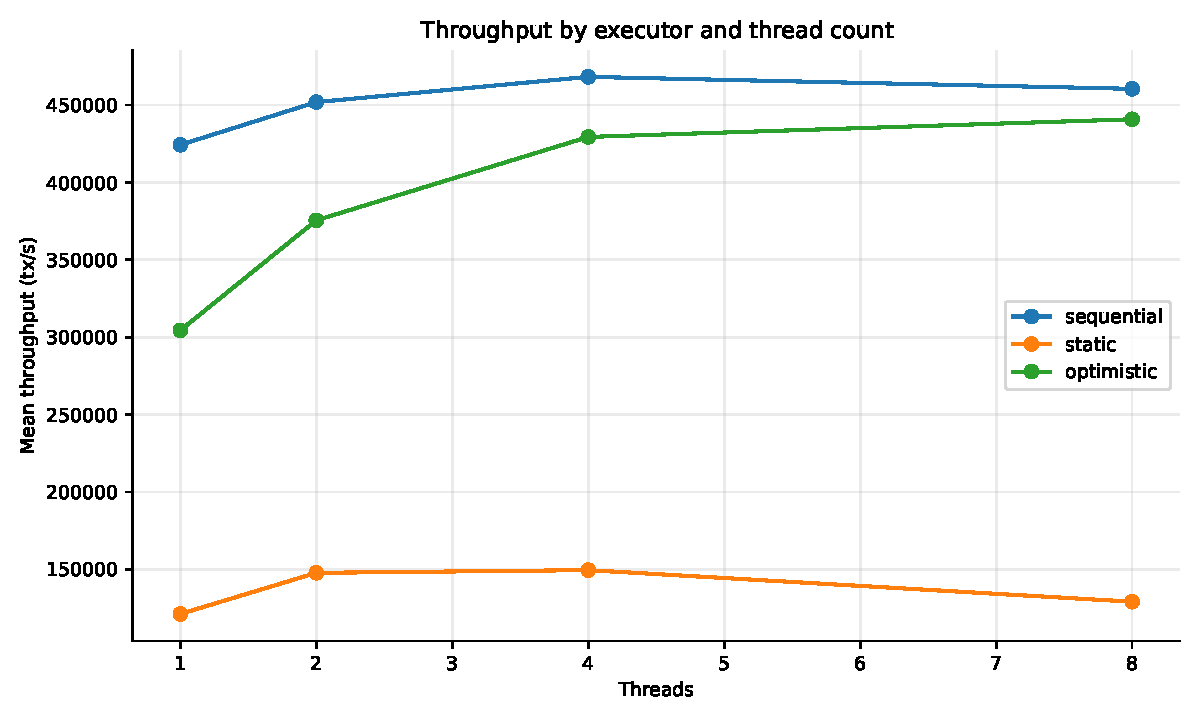
\includegraphics[width=0.9\textwidth]{../results/figures/throughput_by_threads.pdf}
\caption{Mean throughput by executor and thread count.}
\label{fig:throughput}
\end{figure}

Figure~\ref{fig:throughput} shows that the optimistic executor benefited most from additional threads. Its mean throughput increased from 304,392 tx/s at 1 thread to 440,860 tx/s at 8 threads. The best individual run reached 731,729.63 tx/s for the no-conflict workload with 5,000 transactions and 8 threads. The sequential baseline remained comparatively stable because its implementation ignores the thread count and is included as a reference.

\begin{table}
\centering
\caption{Mean throughput by executor and thread count, aggregated across workloads and block sizes.}
\label{tab:throughput}
\begin{tabular}{lrrrr}
\toprule
Executor & 1 thread & 2 threads & 4 threads & 8 threads\\
\midrule
Sequential & 424,334 & 451,956 & 468,282 & 460,522\\
Static & 121,061 & 147,654 & 149,415 & 128,982\\
Optimistic & 304,392 & 375,526 & 429,441 & 440,860\\
\bottomrule
\end{tabular}
\end{table}

\begin{figure}
\centering
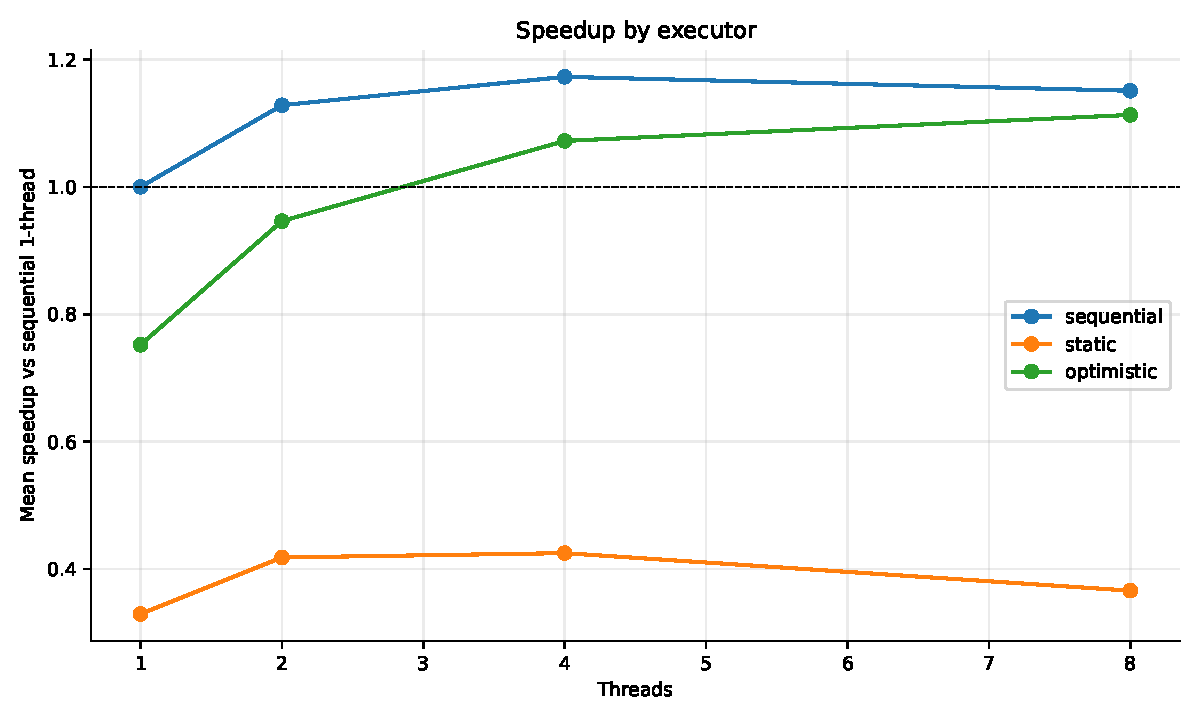
\includegraphics[width=0.9\textwidth]{../results/figures/speedup_by_threads.pdf}
\caption{Speedup relative to the sequential 1-thread baseline.}
\label{fig:speedup}
\end{figure}

The speedup results in Figure~\ref{fig:speedup} show a clear distinction between static and optimistic execution. At 8 threads, optimistic execution had a mean speedup of 1.113 across workload/block-size combinations. Static scheduling had a mean speedup of 0.366 because high-contention and barrier-like workloads produced many small batches and paid scheduling overhead without enough parallel work.

\begin{table}
\centering
\caption{8-thread speedup relative to sequential 1-thread execution.}
\label{tab:speedup}
\begin{tabular}{lrrr}
\toprule
Workload & Block size & Static & Optimistic\\
\midrule
Hotspot & 1,000 & 0.04 & 0.72\\
Hotspot & 5,000 & 0.03 & 0.82\\
No-conflict & 1,000 & 1.34 & 1.59\\
No-conflict & 5,000 & 0.69 & 1.51\\
Private-state & 1,000 & 0.05 & 1.08\\
Private-state & 5,000 & 0.02 & 0.87\\
Token-transfer & 1,000 & 0.72 & 1.47\\
Token-transfer & 5,000 & 0.59 & 1.49\\
Zipfian & 1,000 & 0.11 & 0.75\\
Zipfian & 5,000 & 0.07 & 0.82\\
\bottomrule
\end{tabular}
\end{table}

\begin{figure}
\centering
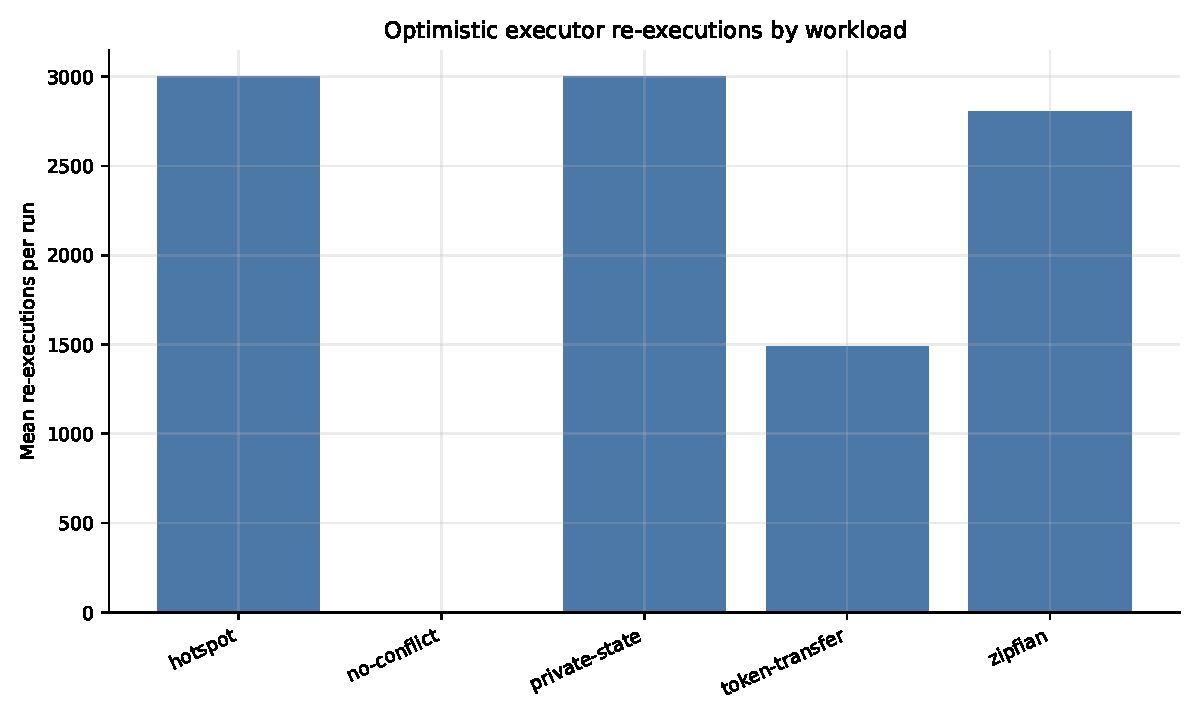
\includegraphics[width=0.9\textwidth]{../results/figures/reexecutions_by_workload.pdf}
\caption{Mean optimistic re-executions by workload.}
\label{fig:reexec}
\end{figure}

Figure~\ref{fig:reexec} explains the optimistic executor's behavior. No-conflict workloads required zero re-executions. Hotspot and private-state workloads required nearly every transaction after the first to re-execute because all transactions touched a shared key: the hotspot account or the commitment root/nullifier-related state. Token-transfer workloads were mixed, with an average of 1,487.83 re-executions across runs, while Zipfian workloads averaged 2,806.33 re-executions because popular accounts produced repeated invalidation.

\begin{figure}
\centering
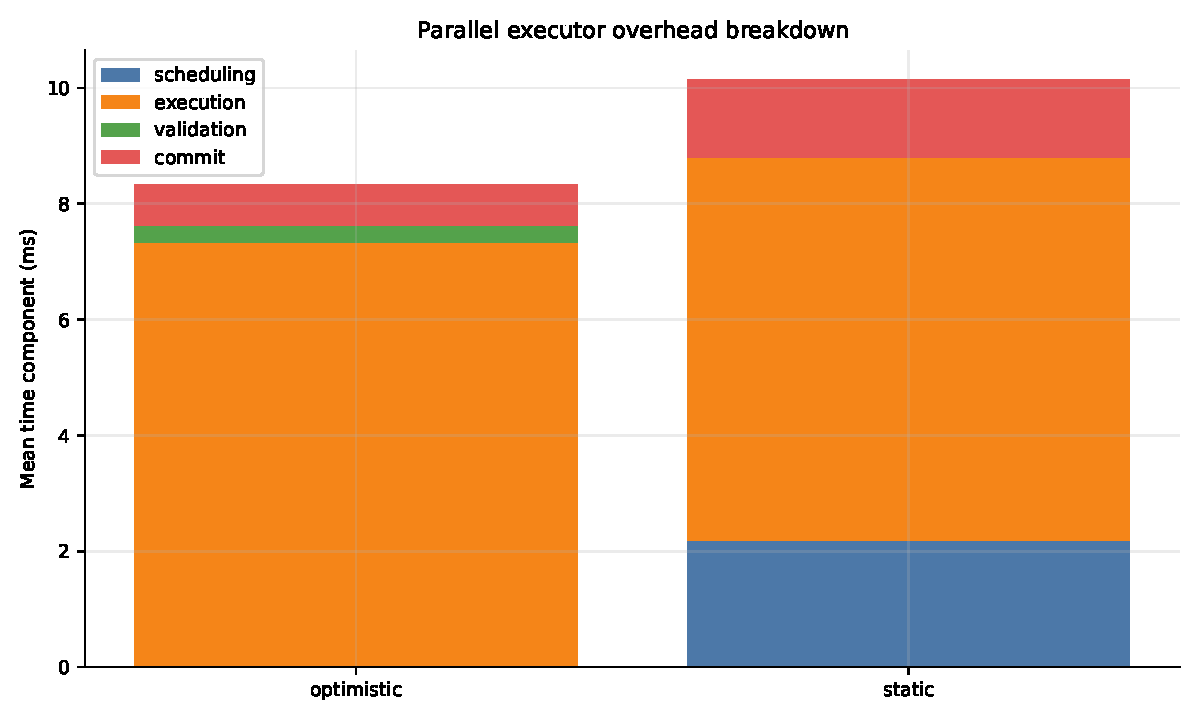
\includegraphics[width=0.9\textwidth]{../results/figures/overhead_breakdown.pdf}
\caption{Mean timing component breakdown for parallel executors.}
\label{fig:overhead}
\end{figure}

Figure~\ref{fig:overhead} shows that static scheduling spent a mean of 2.193 ms in scheduling and 1.352 ms in commit, while optimistic execution spent 0.284 ms in validation and 0.708 ms in commit. Execution time dominated both strategies, but scheduling overhead became visible when batches were small.

\begin{figure}
\centering
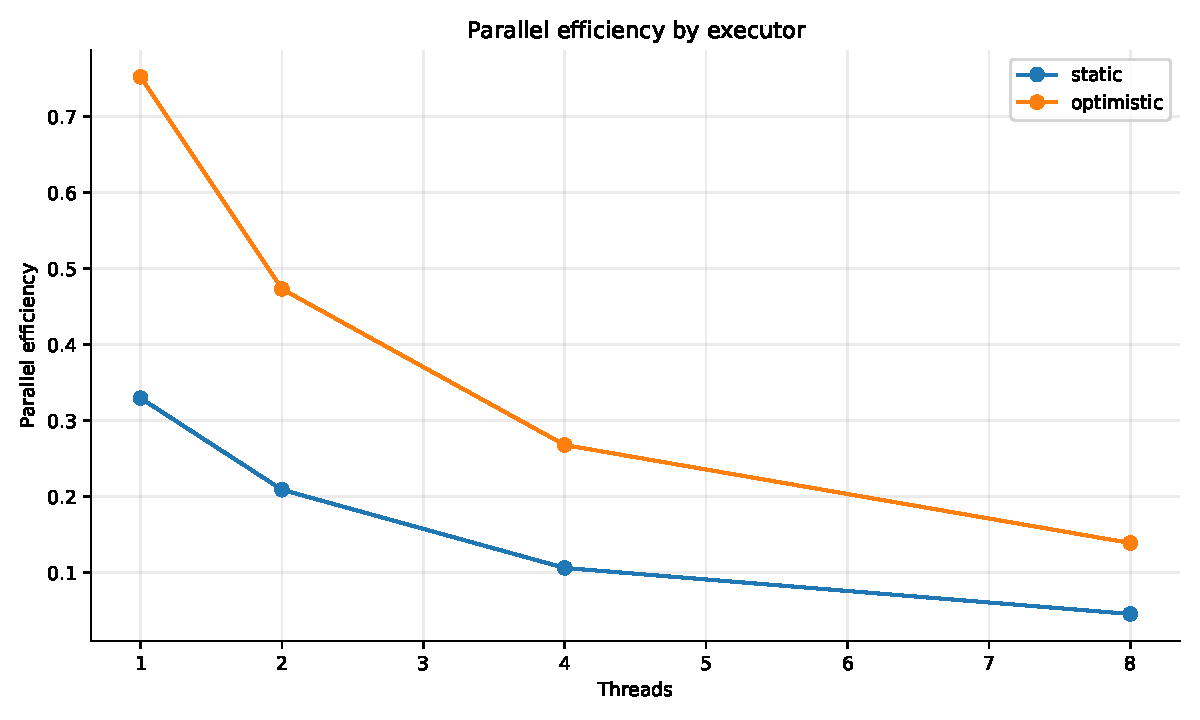
\includegraphics[width=0.9\textwidth]{../results/figures/parallel_efficiency_by_threads.pdf}
\caption{Parallel efficiency for static and optimistic executors.}
\label{fig:efficiency}
\end{figure}

The results support the central hypothesis: deterministic parallel execution helps when enough independent work exists, but contention, validation, re-execution, and ordered commit can remove the benefit. For LEZ-like systems, the safest near-term adaptation is to parallelize stateless validation and computation while preserving ordered state-diff commit.

\subsection{Dual-Environment Kabré Validation}

\begin{center}
\small
\textbf{Table 4.} Local and Kabré benchmark summary.

\vspace{0.5em}
\begin{tabular}{lrrrr}
\toprule
Environment & Rows & Threads & Failures & Best tx/s\\
\midrule
Apple M2 Pro local & 360 & 1--8 & 0 & 731,729.63\\
Kabré Dribe Xeon & 630 & 1--36 & 0 & 583,276.55\\
\bottomrule
\end{tabular}
\end{center}

\begin{figure}
\centering
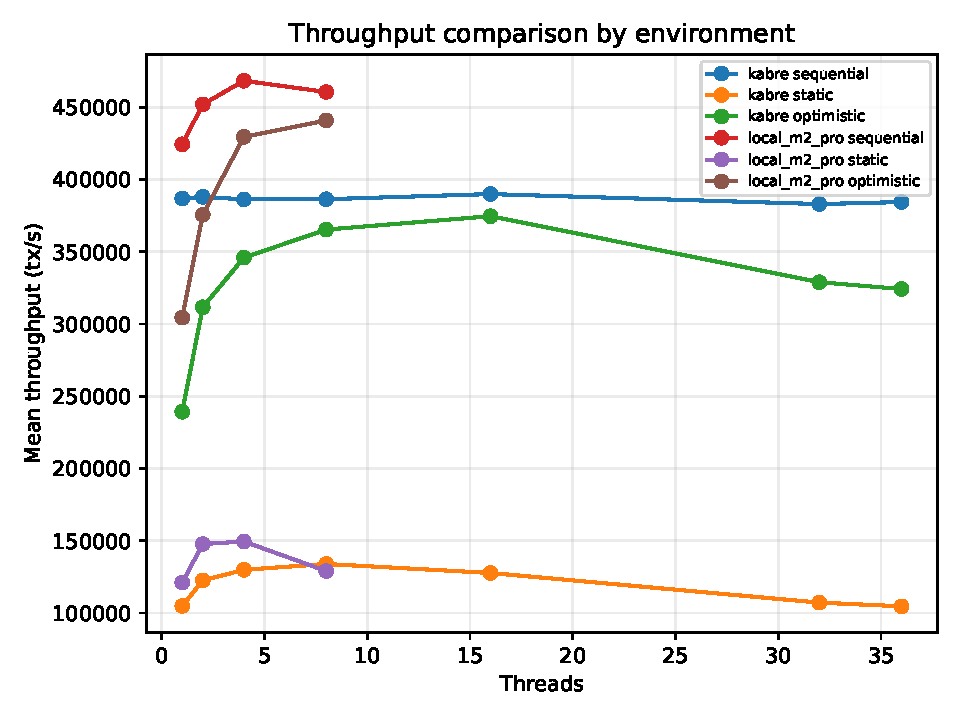
\includegraphics[width=0.9\textwidth]{../results/figures/comparison/environment_throughput_by_threads.pdf}
\caption{Mean throughput comparison between the local Apple M2 Pro run and the Kabré Dribe run.}
\label{fig:environment-comparison}
\end{figure}

Table 4 and Figure~\ref{fig:environment-comparison} show that Kabré is valuable as an additional correctness and scalability environment, but it did not improve the peak throughput of this shared-memory prototype. The best local and Kabré runs were both optimistic no-conflict executions with block size 5,000; the local peak occurred at 8 threads, while the Kabré peak occurred at 16 threads. At common optimistic thread counts, Kabré reached 78.6\% to 83.0\% of the local throughput. Within the Kabré-only high-thread range, optimistic mean throughput increased from 239,213 tx/s at 1 thread to 374,558 tx/s at 16 threads, then declined to 328,869 tx/s at 32 threads and 324,158 tx/s at 36 threads. This suggests that the prototype's overheads, memory behavior, and ordered commit limits dominate after moderate parallelism. The result is still useful: the local run supports the decentralization-oriented claim, while the Kabré run shows that the same semantics remain correct under a larger institutional CPU allocation.

\section{Contributions}

This project makes five concrete contributions:

\begin{enumerate}
\item it organizes related blockchain systems into a taxonomy of declared-access, optimistic, object-centric, asynchronous, and sequential designs;
\item it defines a common conflict model for deterministic block execution over public accounts, nonces, state keys, nullifiers, commitments, program code, and system barriers;
\item it applies the model to Logos Execution Zone and identifies safe parallel validation and ordered-commit boundaries;
\item it implements CAPE as a reproducible Rust benchmark with sequential, static, and optimistic executors;
\item it evaluates the prototype across 990 deterministic benchmark rows in local and Kabré environments and reports measured correctness, throughput, speedup, efficiency, overhead, and re-execution behavior.
\end{enumerate}

\section{Conclusions and Future Work}

CAPE demonstrates that deterministic parallel blockchain execution can preserve sequential semantics while exploiting multicore hardware under favorable dependency patterns. The optimistic executor was the most robust strategy in the experiment, especially on no-conflict and token-transfer workloads. Static scheduling was sensitive to declared conflicts and performed poorly when barriers or shared keys collapsed the schedule into small batches. The Kabré experiment strengthens the correctness result and adds a high-thread stress test, but the local Apple M2 Pro run remained the best peak-throughput environment for this prototype. Therefore, the most accurate conclusion is not that HPC hardware is required, but that deterministic parallel execution is semantically viable and that real performance depends strongly on hardware, contention, and ordered-commit overhead.

For Logos Execution Zone, the practical adaptation path should start with parallel stateless checks, proof or signature verification, transaction classification, and conflict metadata construction. Ordered commit should remain the semantic boundary for public account updates, signer nonces, nullifiers, commitments, program deployments, and global system state. Future work should replace synthetic execution with traces from real LEZ workloads, model proof-verification cost more accurately, evaluate hybrid scheduling, reduce clone overhead with persistent snapshots or versioned storage, and test against adversarial dependency patterns.

\bibliographystyle{splncs04}
\bibliography{references}

\end{document}
